\section{Jonathan}
\subsection{Overview}
\begin{frame}{Jonathan: Overview}
\begin{itemize}
\item Network Structure
\item Constructing the Tables
\item The Resulting Network
\item Implementation of the Network
\end{itemize}
\end{frame}

% \subsection{Network Structure}
% \begin{frame}{Network Structure}
% \begin{itemize}
% \item What does the network look like?
% \item Which features are used and how are their domains defined?
% \end{itemize}
% \begin{figure}
%   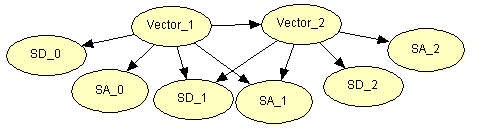
\includegraphics[scale=0.8]{figures/BNDone.PNG}
% \end{figure}
% \end{frame}
\subsection{Network Structure}
\begin{frame}{Network Structure}
\begin{itemize}
\item What does the network look like?
\item Which features are used and how are their domains defined?
\end{itemize}

\begin{figure}
  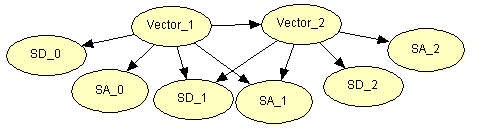
\includegraphics[scale=0.8]{figures/BNDone.PNG}
\end{figure}

\begin{itemize}
  \item Vector - The vector the target is travelling at
  \item SA - The angle at which the target is sensed
  \item SD - The distance to the target
\end{itemize}
\end{frame}

\begin{frame}{Network Structure}
\begin{itemize}
 \item Vector - The vector the target is travelling at
 \item SA - The angle at which the target is sensed
 \item SD - The distance to the target
\end{itemize}

\begin{figure}
  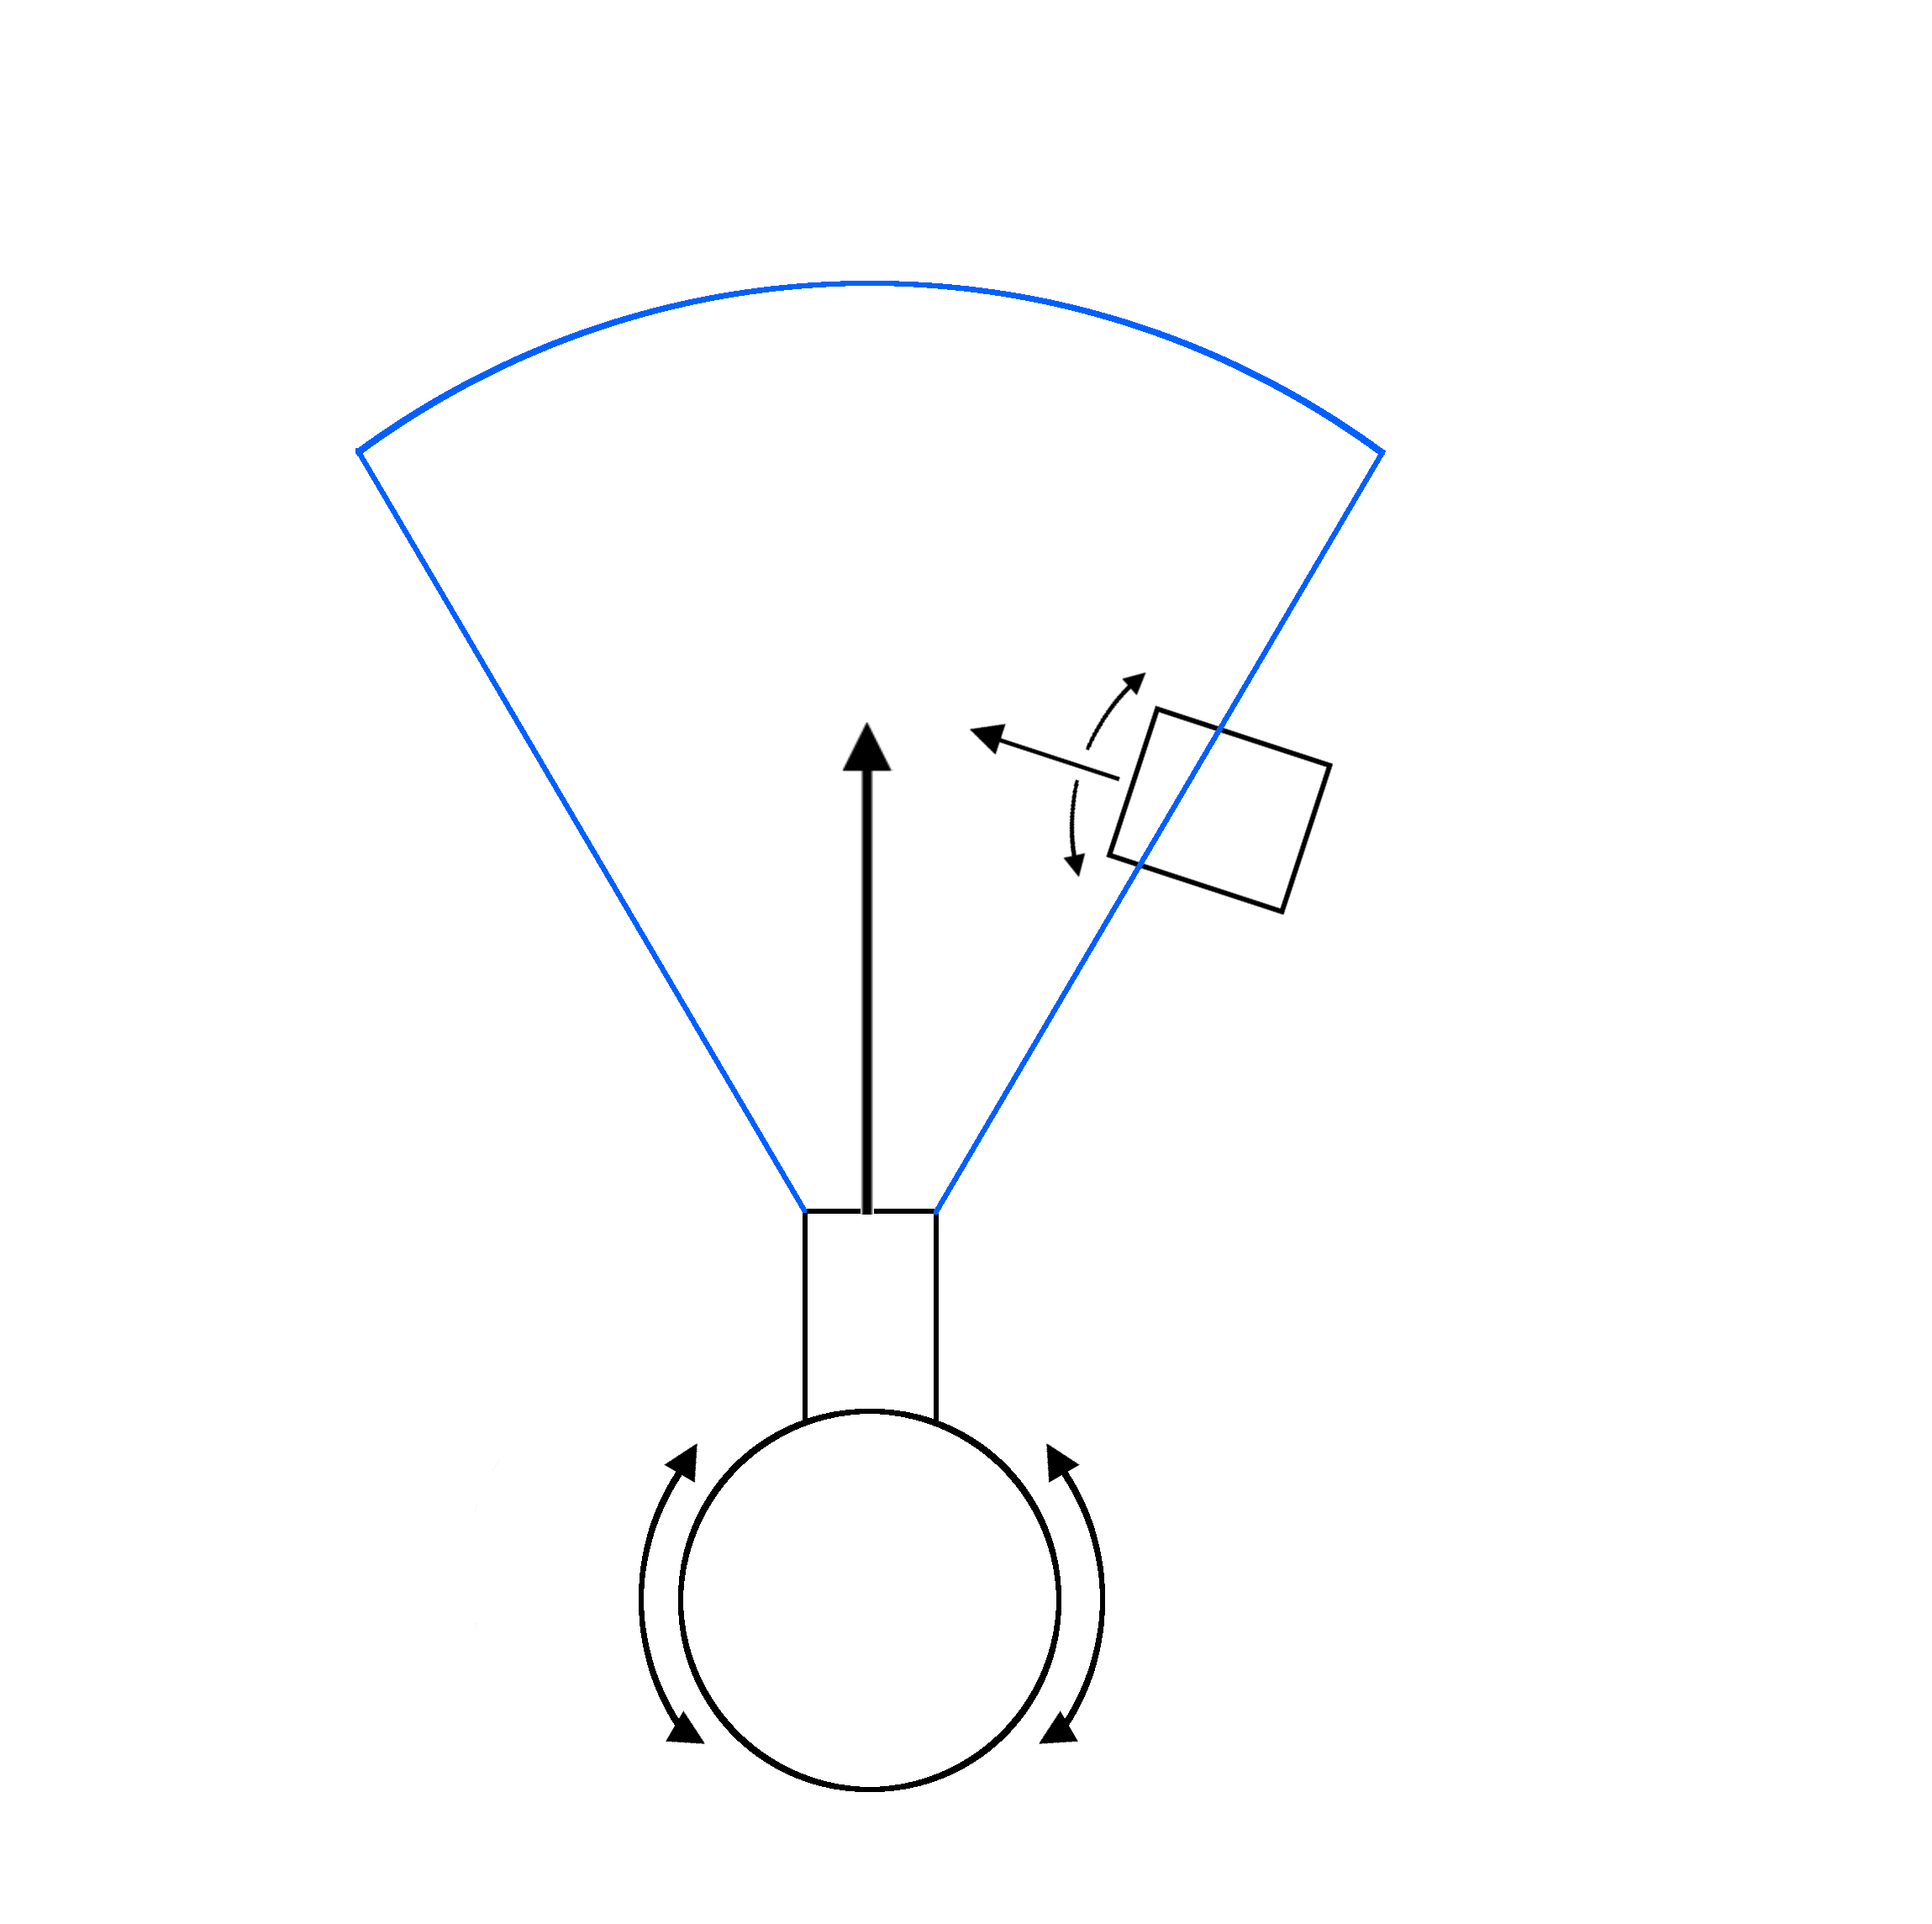
\includegraphics[scale=0.2]{figures/richPic3P5.PNG}
\end{figure}
\end{frame}


\begin{frame}{Network Structure}
\begin{itemize}
 \item Vector - The vector the target is travelling at
 \item SA - The angle at which the target is sensed
 \item SD - The distance to the target
\end{itemize}

\begin{table}
\begin{tabular}{l|l|l}
State & Angle (deg) & Distance (cm) \\ \hline
1     & -30 - 0     & 0 - 60        \\
2     & 0 - 30      & 60 - 75       \\
3     & 30 - 60     & 75 - 90       \\
4     & 60 - 90     & 90 - 105      \\
5     & 90 - 330    & 105 - 255     
\end{tabular}
\end{table}
\end{frame}

\subsection{Constructing the Tables}
\begin{frame}{Constructing the Tables}
\begin{itemize}
\item How was it done? 
\begin{figure}
  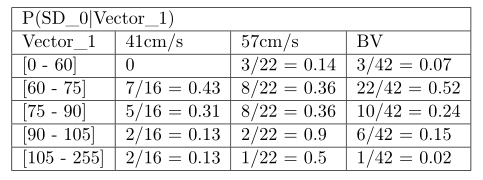
\includegraphics[scale=0.6]{figures/SD0GivenV1.PNG}
\end{figure}

%\item Was the methodology flawed?
\end{itemize}
\end{frame}


\subsection{The Resulting Network}
\begin{frame}{The Resulting Network}
\begin{itemize}
\item Problems with changing vectors
\begin{figure}
  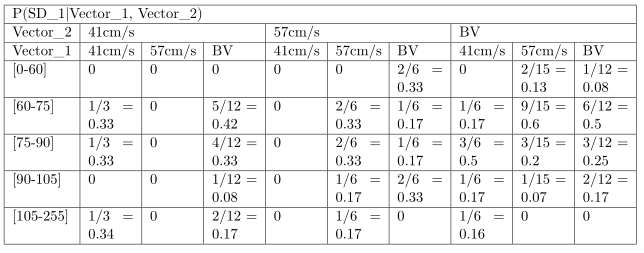
\includegraphics[scale=0.4]{figures/SD1GivenV1V2.PNG}
\end{figure}
\item How can we work around this?
\begin{itemize}
  \item Expanded movement options
  \item Complete rework
  \end{itemize}
\end{itemize}
\end{frame}


\subsection{Implementation of the Belief Network}
\begin{frame}{Implementation of the Belief Network}
\begin{itemize}
\item Have a scaled down version of the network on the NXT
\item Set up a connection to a PC for processing power
\begin{itemize}
   \item Bluetooth vs Serial connection
   \item Defeats the purpose of an embedded system?
   \end{itemize}
\end{itemize}
\end{frame}
